\documentclass[crop,tikz]{standalone}

\usetikzlibrary{positioning}

\begin{document}
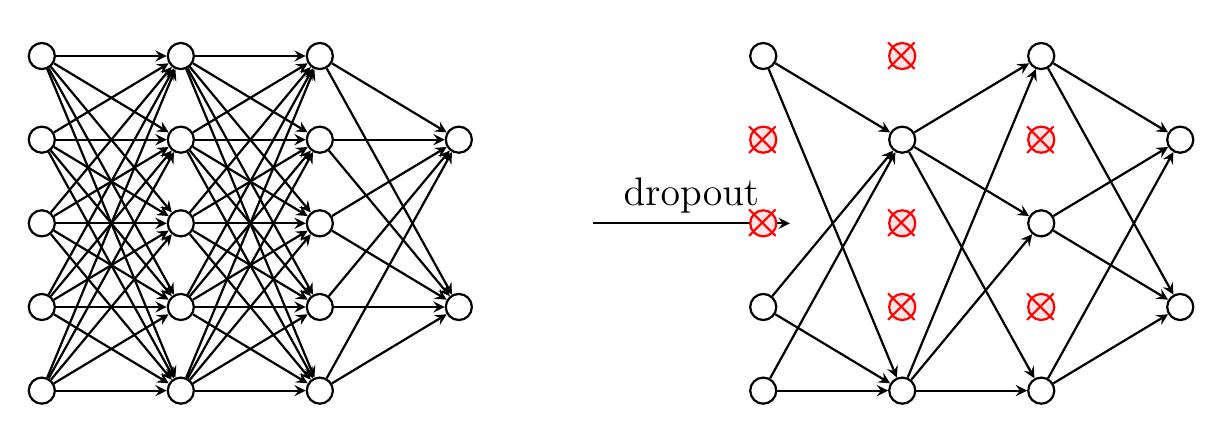
\begin{tikzpicture}

	\node[circle, draw, thick] (i1) {};
	\node[circle, draw, thick, above=2em of i1] (i2) {};
	\node[circle, draw, thick, above=2em of i2] (i3) {};
	\node[circle, draw, thick, below=2em of i1] (i4) {};
	\node[circle, draw, thick, below=2em of i4] (i5) {};
	
	\node[circle, draw, thick, right=4em of i1] (h1) {};
	\node[circle, draw, thick, right=4em of i2] (h2) {};
	\node[circle, draw, thick, right=4em of i3] (h3) {};
	\node[circle, draw, thick, right=4em of i4] (h4) {};
	\node[circle, draw, thick, right=4em of i5] (h5) {};
	
	\node[circle, draw, thick, right=4em of h1] (hh1) {};
	\node[circle, draw, thick, right=4em of h2] (hh2) {};
	\node[circle, draw, thick, right=4em of h3] (hh3) {};
	\node[circle, draw, thick, right=4em of h4] (hh4) {};
	\node[circle, draw, thick, right=4em of h5] (hh5) {};
	
	\node[circle, draw, thick, right=4em of hh2] (o1) {};
	\node[circle, draw, thick, right=4em of hh4] (o2) {};
	
	\draw[-stealth, thick] (i1) -- (h1);
	\draw[-stealth, thick] (i1) -- (h2);
	\draw[-stealth, thick] (i1) -- (h3);
	\draw[-stealth, thick] (i1) -- (h4);
	\draw[-stealth, thick] (i1) -- (h5);
	\draw[-stealth, thick] (i2) -- (h1);
	\draw[-stealth, thick] (i2) -- (h2);
	\draw[-stealth, thick] (i2) -- (h3);
	\draw[-stealth, thick] (i2) -- (h4);
	\draw[-stealth, thick] (i2) -- (h5);
	\draw[-stealth, thick] (i3) -- (h1);
	\draw[-stealth, thick] (i3) -- (h2);
	\draw[-stealth, thick] (i3) -- (h3);
	\draw[-stealth, thick] (i3) -- (h4);
	\draw[-stealth, thick] (i3) -- (h5);
	\draw[-stealth, thick] (i4) -- (h1);
	\draw[-stealth, thick] (i4) -- (h2);
	\draw[-stealth, thick] (i4) -- (h3);
	\draw[-stealth, thick] (i4) -- (h4);
	\draw[-stealth, thick] (i4) -- (h5);
	\draw[-stealth, thick] (i5) -- (h1);
	\draw[-stealth, thick] (i5) -- (h2);
	\draw[-stealth, thick] (i5) -- (h3);
	\draw[-stealth, thick] (i5) -- (h4);
	\draw[-stealth, thick] (i5) -- (h5);
	
	\draw[-stealth, thick] (h1) -- (hh1);
	\draw[-stealth, thick] (h1) -- (hh2);
	\draw[-stealth, thick] (h1) -- (hh3);
	\draw[-stealth, thick] (h1) -- (hh4);
	\draw[-stealth, thick] (h1) -- (hh5);
	\draw[-stealth, thick] (h2) -- (hh1);
	\draw[-stealth, thick] (h2) -- (hh2);
	\draw[-stealth, thick] (h2) -- (hh3);
	\draw[-stealth, thick] (h2) -- (hh4);
	\draw[-stealth, thick] (h2) -- (hh5);
	\draw[-stealth, thick] (h3) -- (hh1);
	\draw[-stealth, thick] (h3) -- (hh2);
	\draw[-stealth, thick] (h3) -- (hh3);
	\draw[-stealth, thick] (h3) -- (hh4);
	\draw[-stealth, thick] (h3) -- (hh5);
	\draw[-stealth, thick] (h4) -- (hh1);
	\draw[-stealth, thick] (h4) -- (hh2);
	\draw[-stealth, thick] (h4) -- (hh3);
	\draw[-stealth, thick] (h4) -- (hh4);
	\draw[-stealth, thick] (h4) -- (hh5);
	\draw[-stealth, thick] (h5) -- (hh1);
	\draw[-stealth, thick] (h5) -- (hh2);
	\draw[-stealth, thick] (h5) -- (hh3);
	\draw[-stealth, thick] (h5) -- (hh4);
	\draw[-stealth, thick] (h5) -- (hh5);
	
	
	\draw[-stealth, thick] (hh1) -- (o1);
	\draw[-stealth, thick] (hh1) -- (o2);
	\draw[-stealth, thick] (hh2) -- (o1);
	\draw[-stealth, thick] (hh2) -- (o2);
	\draw[-stealth, thick] (hh3) -- (o1);
	\draw[-stealth, thick] (hh3) -- (o2);
	\draw[-stealth, thick] (hh4) -- (o1);
	\draw[-stealth, thick] (hh4) -- (o2);
	\draw[-stealth, thick] (hh5) -- (o1);
	\draw[-stealth, thick] (hh5) -- (o2);
	
	\draw[-stealth, thick] (7,0) -- node[above,font=\Large] {dropout} (9.5, 0);
	
	
	%%% Boundary %%%
	
	\node[circle, draw, thick, red, fill=red!10, right=15em of hh1] (i1) {};
	\node[circle, draw, thick, red, fill=red!10, above=2em of i1] (i2) {};
	\node[circle, draw, thick, above=2em of i2] (i3) {};
	\node[circle, draw, thick, below=2em of i1] (i4) {};
	\node[circle, draw, thick, below=2em of i4] (i5) {};
	
	\node[red,font=\huge] (icr) at (i1) {$\times$};
	\node[red,font=\huge] (icr) at (i2) {$\times$};
	
	\node[circle, draw, thick, red, fill=red!10, right=4em of i1] (h1) {};
	\node[circle, draw, thick, right=4em of i2] (h2) {};
	\node[circle, draw, thick, red, fill=red!10, right=4em of i3] (h3) {};
	\node[circle, draw, thick, red, fill=red!10, right=4em of i4] (h4) {};
	\node[circle, draw, thick, right=4em of i5] (h5) {};
	
	\node[red,font=\huge] (icr) at (h1) {$\times$};
	\node[red,font=\huge] (icr) at (h3) {$\times$};
	\node[red,font=\huge] (icr) at (h4) {$\times$};
	
	\node[circle, draw, thick, right=4em of h1] (hh1) {};
	\node[circle, draw, thick, red, fill=red!10, right=4em of h2] (hh2) {};
	\node[circle, draw, thick, right=4em of h3] (hh3) {};
	\node[circle, draw, thick, red, fill=red!10, right=4em of h4] (hh4) {};
	\node[circle, draw, thick, right=4em of h5] (hh5) {};
	
	\node[red,font=\huge] (icr) at (hh2) {$\times$};
	\node[red,font=\huge] (icr) at (hh4) {$\times$};
	
	\node[circle, draw, thick, right=4em of hh2] (o1) {};
	\node[circle, draw, thick, right=4em of hh4] (o2) {};
	
	\draw[-stealth, thick] (i3) -- (h2);
	\draw[-stealth, thick] (i3) -- (h5);
	\draw[-stealth, thick] (i4) -- (h2);
	\draw[-stealth, thick] (i4) -- (h5);
	\draw[-stealth, thick] (i5) -- (h2);
	\draw[-stealth, thick] (i5) -- (h5);
	
	\draw[-stealth, thick] (h2) -- (hh1);
	\draw[-stealth, thick] (h2) -- (hh3);
	\draw[-stealth, thick] (h2) -- (hh5);
	\draw[-stealth, thick] (h5) -- (hh1);
	\draw[-stealth, thick] (h5) -- (hh3);
	\draw[-stealth, thick] (h5) -- (hh5);
	
	\draw[-stealth, thick] (hh1) -- (o1);
	\draw[-stealth, thick] (hh1) -- (o2);
	\draw[-stealth, thick] (hh3) -- (o1);
	\draw[-stealth, thick] (hh3) -- (o2);
	\draw[-stealth, thick] (hh5) -- (o1);
	\draw[-stealth, thick] (hh5) -- (o2);

\end{tikzpicture}
\end{document}
